%\documentclass[handout]{beamer}
\documentclass[handout,hyperref={colorlinks=true}]{beamer}
%\documentclass[hyperref={colorlinks=true}]{beamer}



\mode<all>
{
  \usetheme{Berkeley}
  % oder ...
  
  \setbeamercovered{transparent}
  % oder auch nicht
}
\usepackage{newtxtext,newtxmath}
%\usepackage{mathptmx}
\usepackage[spanish]{babel}
\usepackage[latin1]{inputenc}
\usepackage{times}
%\usepackage[T1]{fontenc}
\usepackage{amssymb,amsmath}
\usepackage{enumerate}
\usepackage{verbatim}
\usepackage{array}
\usepackage{wrapfig}
\usepackage{bm}
\usepackage{url}
\usepackage{multirow}
%\usepackage{animate,movie15}
%\usepackage{times}
\usepackage{empheq}
%\usepackage[spanish]{babel}
%\usepackage[utf8x]{inputenc}
%\usepackage{times}
%\usepackage[T1]{fontenc}
%\usepackage{amssymb,amsmath}%,amsthm}
\usepackage{enumerate}
\usepackage{verbatim}
%\usepackage{ esint }
\usepackage{pdfsync}
%\usepackage{theorem}
%\usepackage{pst-all}
%\usepackage{pstricks-add}
\usepackage{array}
%\usepackage[T1]{fontenc}
\usepackage{animate}
%\usepackage{media9}
%\usepackage{movie15}
\usepackage{xparse}
\usepackage{multirow}
%\usepackage{listings}
%\usepackage{ wasysym }
%\usepackage{sagetex}
\usepackage{hyperref}
%\usepackage[margin=1.5cm]{geometry}
\usepackage{tabularx}
\usepackage{tikz}
\usetikzlibrary{backgrounds}
\usetikzlibrary{trees,positioning,arrows}
\usetikzlibrary{mindmap}
%% newcommand
\newtheorem{thm}{Teorema}
\newcommand{\orlnor}{\|_{L^{\Phi}}}
\newcommand{\lurnor}{\|^{*}_{L^{\Phi}}}
\newcommand{\linf}{\|_{L^{\infty}}}
\newcommand{\lphi}{L^{\Phi}}
\newcommand{\lpsi}{L^{\Psi}}
\newcommand{\ephi}{E^{\Phi}}
\newcommand{\claseor}{\widetilde{L}^{\Phi}}
\newcommand{\wphi}{W^{1}\lphi}
\newcommand{\sobnor}{\|_{W^{1}\lphi}}
\newcommand{\domi}{W^{1}\left(\lphi,\Pi\left(\ephi,1\right)\right)}
\newcommand{\com}{\mathbb{C}}
\newcommand{\dis}{\mathbb{D}}
\newcommand{\xb}{\bm{x}}
\newcommand{\rr}{\mathbb{R}}
%\renewcommand{\b}[1]{\boldsymbol{#1}}
\renewcommand{\b}[1]{\vec{#1}}

\definecolor{myblue}{rgb}{.8, .8, 1}
\newlength\mytemplen
\newsavebox\mytempbox
\makeatletter
\newcommand\mybluebox{%
    \@ifnextchar[%]
       {\@mybluebox}%
       {\@mybluebox[0pt]}}

\def\@mybluebox[#1]{%
    \@ifnextchar[%]
       {\@@mybluebox[#1]}%
       {\@@mybluebox[#1][0pt]}}

\def\@@mybluebox[#1][#2]#3{
    \sbox\mytempbox{#3}%
    \mytemplen\ht\mytempbox
    \advance\mytemplen #1\relax
    \ht\mytempbox\mytemplen
    \mytemplen\dp\mytempbox
    \advance\mytemplen #2\relax
    \dp\mytempbox\mytemplen
    \colorbox{myblue}{\hspace{1em}\usebox{\mytempbox}\hspace{1em}}}

\makeatother
\DeclareDocumentCommand\boxedeq{ m g }{%
    {\begin{empheq}[box={\mybluebox[2pt][2pt]}]{equation}% #1%
        \IfNoValueF {#2} {\label{#2}}%
       #1
       \end{empheq}
    }%
}



\title[Soluciones sim�tricas]
{%
Soluciones sim�tricas del problema de los $N$-cuerpos
}
\author[F. Mazzone]{Fernando Mazzone\\
 }
\institute[UNRC-CONICET]{Depto de Matem�tica, Facultad de Ciencias Exactas, F�sico-Qu�micas y Naturales, Universidad Nacional de R�o Cuarto\\
CONICET\\

\includegraphics[scale=0.2]{unrc.jpg}\hspace{1cm} 
\includegraphics[scale=0.4]{logoC.png} }
\date[8/4/2016]{Seminario de Investigaci�n en Matem�tica Aplicada}
\subject{Asteroides}

\begin{document}
\begin{frame}
  \maketitle
\end{frame}




\section{Problema de los $N$-cuerpos}
\subsection{Ecuaci�n}
\begin{frame}{Problema}

\onslide<+->\begin{block}{Sistema f�sico}

\begin{description}
\item[Espacio:] Espacio euclideano $d$ dimensional $d\geq 2$ ($\rr^d$).
\item[Objetos:] $N$-puntos de masas $m_1,m_2,\ldots,m_N$,
\item[Variables:] tiempo $t$, posiciones $\b{r}_i=\b{r}_i(t)\in \rr^d$, $i=1,\ldots,N$,
 \item[Fuerzas:] gravitacionales,
 \item[Leyes f�sicas:] Mec�nica Newtoniana: Segunda Ley y Ley de gravitaci�n universal.
 
\end{description}
 \end{block}
 \end{frame} 



\begin{frame}{Ecuaci�n de los $N$-cuerpos}

\onslide<+->\begin{block}{Ecuaciones $N$-cuerpos}
\[\b{r}''_i(t)=G\sum_{j\neq i}m_j\frac{\b{r}_j-\b{r}_i}{\|\b{r}_j-\b{r}_i\|^3}.\]
$G$ constante gravitaci�n universal, supondremos $G=1$.
\end{block}



 \end{frame} 



\begin{frame}{Problemas: mapa conceptual}
\begin{center}
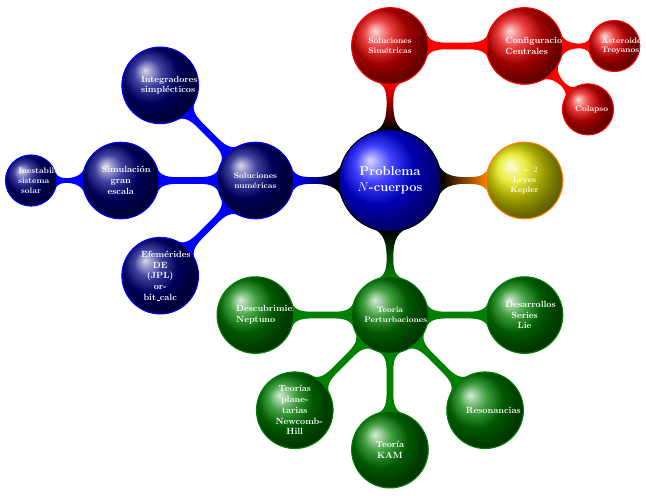
\includegraphics[scale=.43]{diagrama.png}
\end{center}


\end{frame} 
 

 
\begin{frame}{Notaciones}
\[
  \begin{split}
    \b{r}&=(\b{r}_1,\ldots,\b{r}_N)\in\rr^{dN},\quad\text{Vector configuraci�n},\\
    r_{ij}&=\|\b{r}_i-\b{r}_j\|,\quad\text{distancias relativas},\\
    M&=
       \begin{pmatrix}
	  M_1           & 0_{d\times d} &\cdots & 0_{d\times d}\\
	  0_{d\times d} & M_2           &\cdots & 0_{d\times d}\\
	  \vdots        & \ddots         &      &\vdots        \\
	  0_{d\times d} & \cdots         &      & M_N           \\
       \end{pmatrix},\,
       M_j=\begin{pmatrix}
            m_j     &  \cdots &  0   \\
           \vdots  & \ddots  & \vdots  \\
              0     &     \cdots     & m_j\\                
           \end{pmatrix}\in\rr^{d\times d}
       \\
    U(\b{r})&=      \sum_{i<j}\frac{m_im_j}{r_{ij}}\quad\text{Potencial newtoniano}\\
    \Delta&=\{\b{r}_j=\b{r}_j| \text{ para algunos } i\neq j\},\\ 
    \rr^{dN}-\Delta &\quad\text{ Espacio de configuraciones }.\\ 
  \end{split}
\]

\end{frame} 


 
\begin{frame}{Notaciones}
\[
  \begin{split}
   \b{v}&=\b{r}'\quad\text{(Velocidades)}\\
   K(\b{v})&=\frac12\b{v}\cdot M\b{v}=\frac12\sum_{j=1}^N m_j\|\b{v}_j\|^2,\quad \text{(Energ�a  cin�tica)}\\
   \b{c}&=\frac{1}{m}\sum_{j=1}^Nm_j\b{r}_j,\quad\text{con }m:=\sum_{j=1}^Nm_j\quad\text{(Centro masas)}\\
     \b{p}&=\sum_{j=1}^Nm_j\b{v}_j,\quad\text{(momento total)}\\
     \omega_{kl}&=\sum_{j=1}^Nm_j \left(\b{r}_{jk}\b{v}_{jl}-\b{r}_{jl}\b{v}_{jk}\right),\,\, \text{(Momento angular total $\omega^t=-\omega$)}
  \end{split}
\]

\[\boxed{M\b{r}''(t)=\nabla U(\b{r})},\quad \text{(Ecuaci�n $N$-cuerpos)}\]

\end{frame} 

\begin{frame}{Notaciones}
\[
  \begin{split}
   I(\b{r})&= \frac12(\b{r}-\b{c})\cdot M(\b{r}-\b{c})=\frac12\sum_{j=1}^N m_j\|\b{r}_j-\b{c}\|^2,\\ &\text{(Momento de inercia)}\\
  \end{split}
\]

\boxedeq{M\b{r}''(t)=\nabla U(\b{r}),\,\text{(Ecuaci�n $N$-cuerpos)}}{}

\end{frame} 


 
  \subsection{Simetr�as}
 \begin{frame}{ \begin{tabular}{cc} \multirow{2}{*}{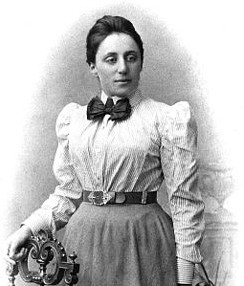
\includegraphics[scale=.5]{Noether.jpg}} & Simetr�as e integrales primeras \\  &(Emmy Noether)\\\end{tabular}}
 \begin{itemize}
  \item<+-> \textbf{Simetr�a por traslaciones} ($\b{r}_j\rightarrow \b{r}_j+\b{v}_0t+\b{c}_0$, $\b{c}_0,\b{v}_0\in\rr^d$) $\Rightarrow$ \fbox{conservaci�n $\b{p}=\b{c}'$}  $\Rightarrow$ movimiento rectilineo uniforme de $\b{c}$ 
    \item<+-> \textbf{Simetr�a por rotaciones} ($\b{r}_j\rightarrow Q\b{r}_j$, $Q\in O(d)$) $\Rightarrow$ \fbox{conservaci�n $\omega$}
    \item<+-> La \textbf{energ�a total} $H:\underset{\text{Espacio fases}}{\underbrace{\left(\rr^d-\Delta\right)\times\rr^d}}\to  \rr$,
    \[H(\b{r},\b{v})=K(\b{v})-U(\b{r}),\]
    se conserva
  
 \end{itemize}



\end{frame} 

 
 
 
\section{Configuraciones centrales}
\begin{frame}{Configuraciones centrales (CC)}
\onslide<+->\begin{block}{Definici�n} Una configuraci�n de puntos masa, con masas $m_1,\ldots,m_N$ y posiciones $\b{r}_1,\ldots,\b{r}_N$ es central si existe $\lambda\in\rr$ tal que
\[\nabla U(\b{r})+\lambda M(\b{r}-\b{c})=\nabla U(\b{r})+\lambda \nabla I(\b{r}-\b{c})=0.\]
 
\end{block}
\onslide<+->\textbf{Observaci�n:} En una configuraci�n central el vector aceleraci�n sobre cada cuerpo apunta hacia $\b{c}$  y es proporcional a la distancia a $\b{c}$.

\end{frame} 

\begin{frame}{Existencia de CC}
\begin{itemize}
 \item<+-> Para masas arbitrarias la existencia es poco clara. 
 \item<+-> \textbf{Soluciones sencillas} Si todas las masas son iguales $m_1=m_2=\cdots=m_N$ podemos ponerlas como v�rtices de un pol�topo, pol�gono regular del plano, poliedro regular (s�lido plat�nico), etc. Claramente la configuraci�n es central
\item<+-> Notoriamente en el caso del regular $d$-simplex, tri�ngulo equil�tero, tetraedro, etc, tenemos CC independientemente de las masas.
\end{itemize}

\onslide

\end{frame} 

\end{document}